\section{HISTORIA DE LA CRIPTOGRAFÍA}
\begin{frame}{HISTORIA DE LA CRIPTOGRAFÍA}
	\begin{itemize}
	\item Khnumhotep II - Egipto, India.
	\item Cifrado de César, 100 A.C.
	\item Cifrado de Vigenere, Siglo 16.
	\item La máquina Enigma.
	\end{itemize}
    \centering 158,962,555,217,826,360,000 
    \begin{figure}
    	\centering
        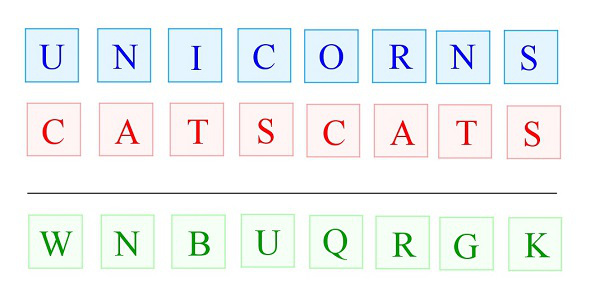
\includegraphics[scale=0.5]{vieCip.jpg}
        \caption{Ejemplo del Cifrado de Vigenere\footnotemark{}}
    \end{figure}
    \vspace{-3mm}\footnotetext{\bibentry{vige}}
\end{frame}
%%%%%%%%%%%%%%%%%%%%%%%%%%%%%%%%%%%%%%%%%%%%%%%%%%%%
\section{TIPOS DE CRIPTOGRAFÍA}
\subsection{Simétrica}
\begin{frame}{TIPOS DE CRIPTOGRAFÍA}
	\framesubtitle{Simétrica}
    Se utiliza la misma llave (privada) para cifrar y descifrar el mensaje.
    \begin{figure}
    	\centering
        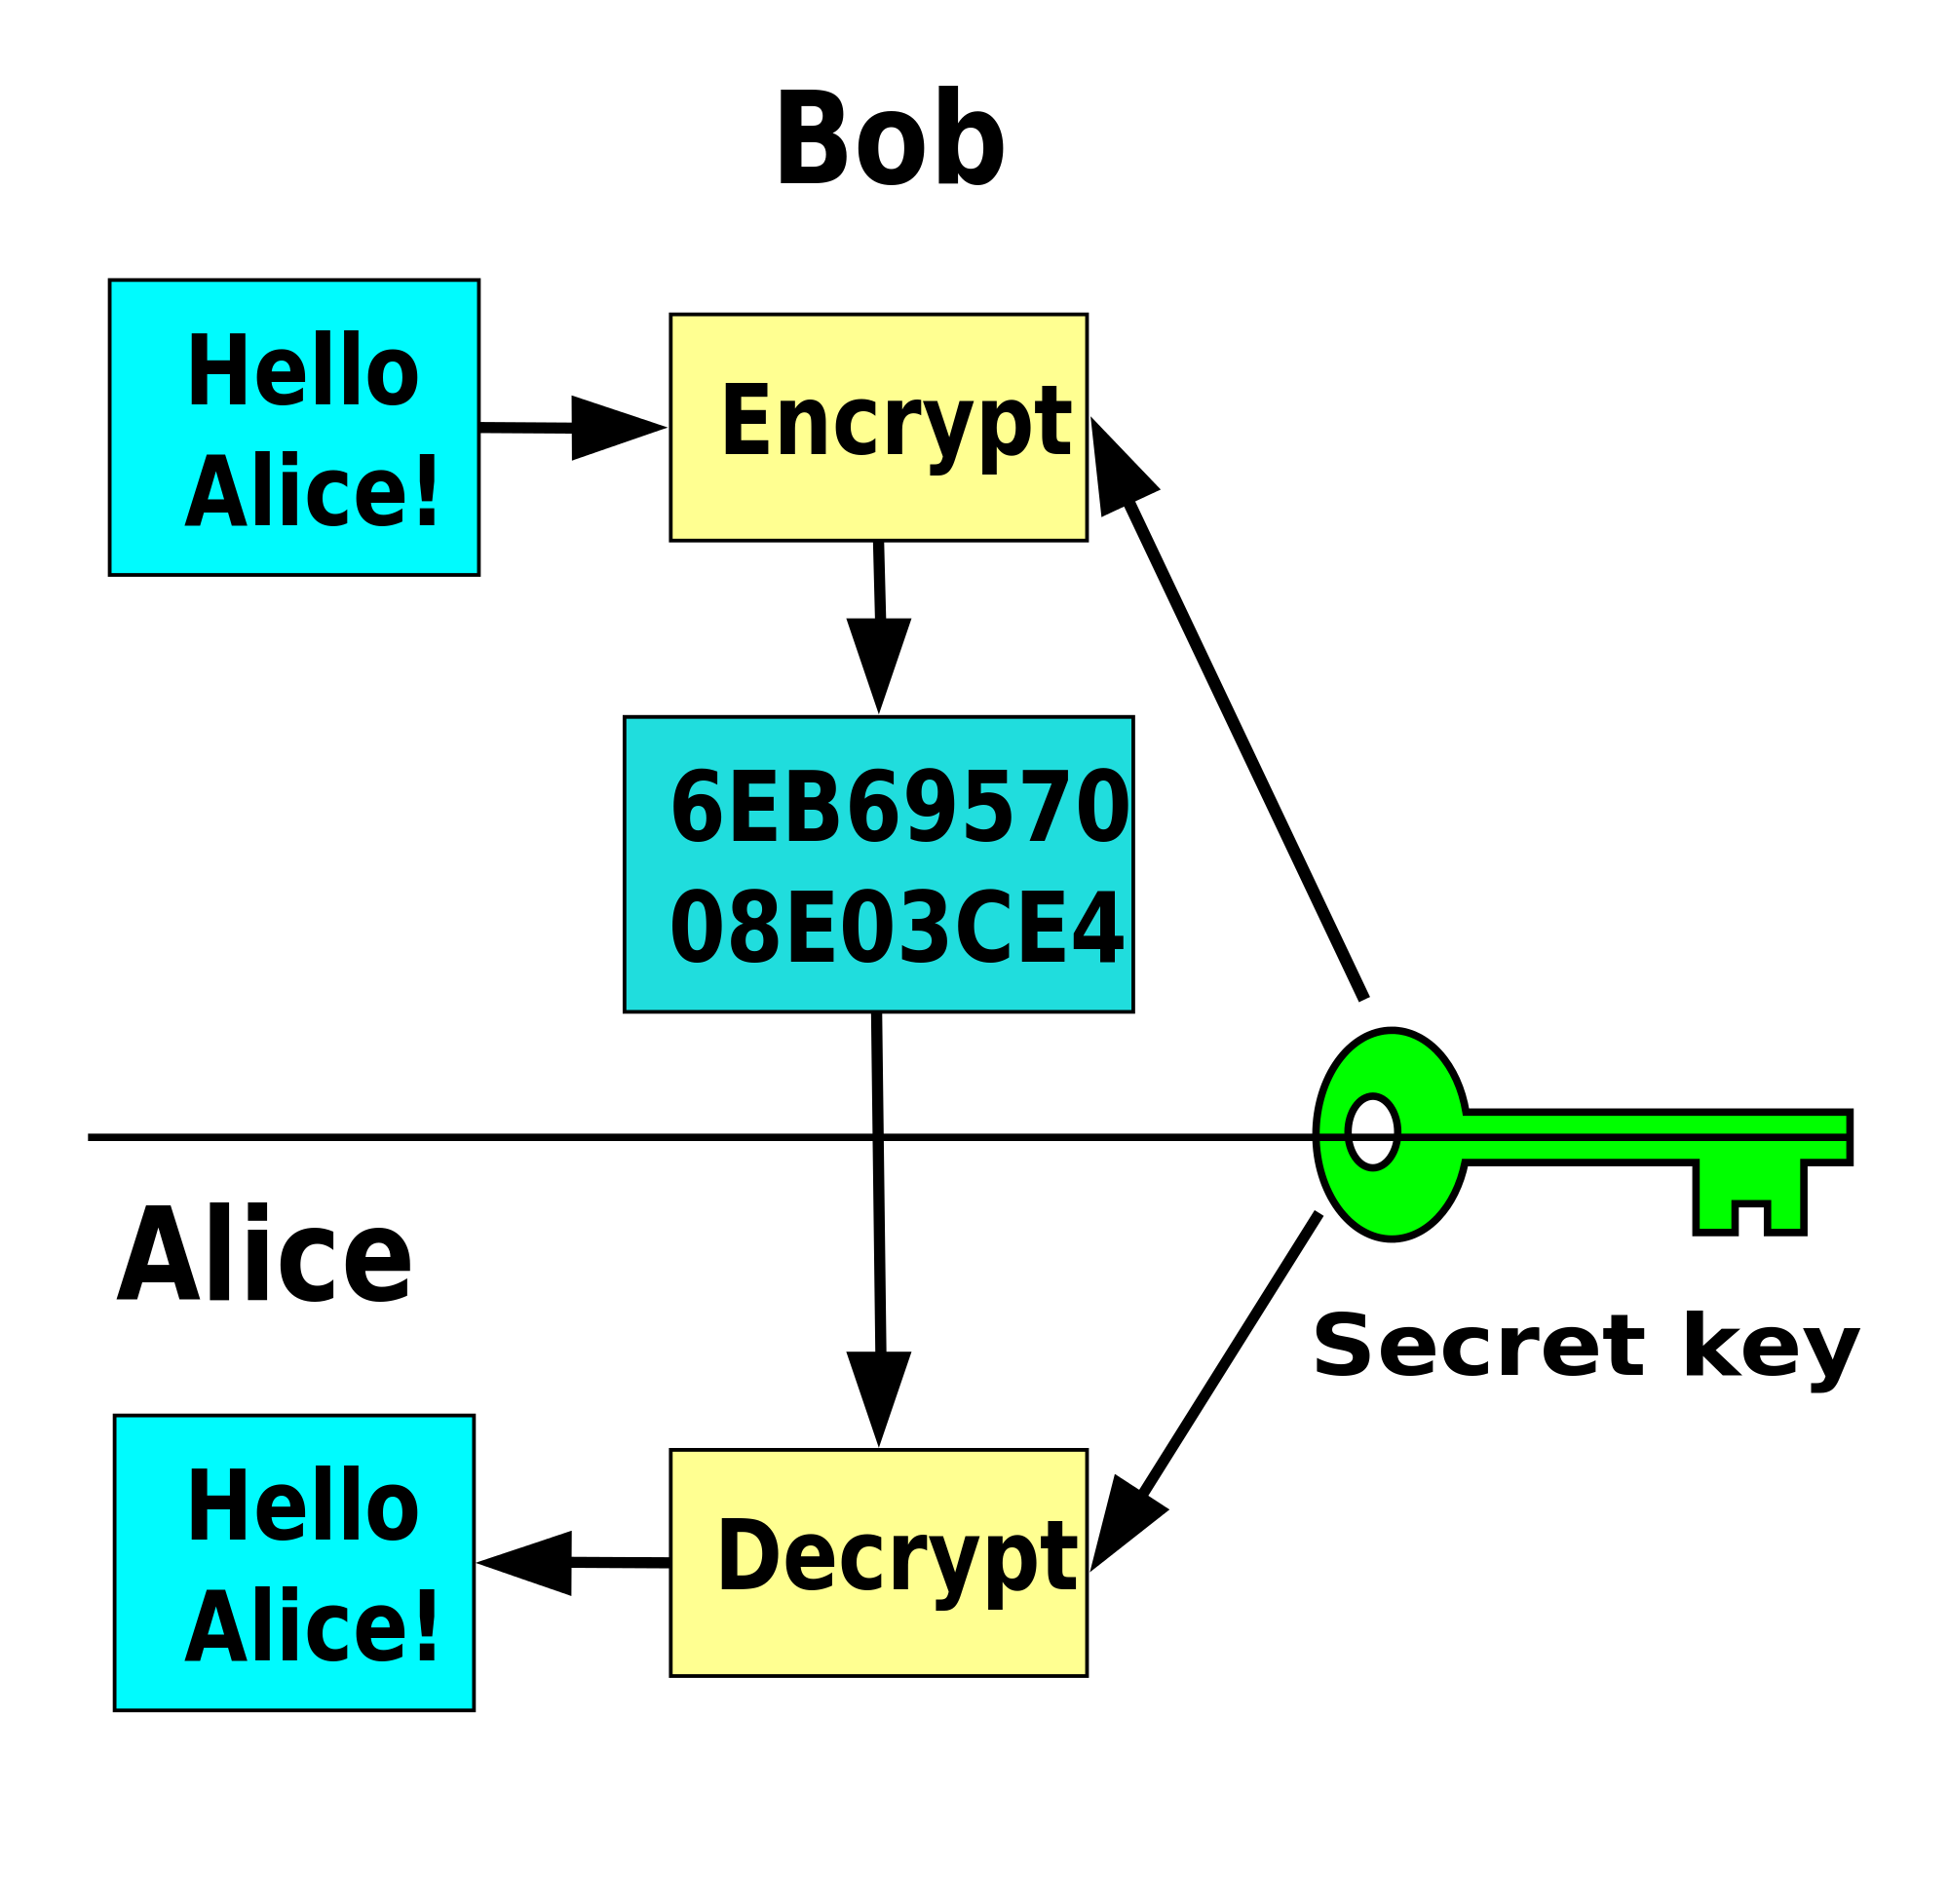
\includegraphics[scale=0.075]{symmetric.png}
        \caption{Ilustración de criptografía simétrica\footnotemark{}}
    \end{figure}
    \vspace{-0.5cm}\footnotetext{\bibentry{symm}}
\end{frame}
%%%%%%%%%%%%%%%%%%%%%%%%%%%%%%%%%%%%%%%%%%%%%%%%%%%%%
\subsection{Antisimétrica}
\begin{frame}{TIPOS DE CRIPTOGRAFÍA}
	\framesubtitle{Antisimétrica}
    Hay dos llaves, una privada y otra pública. Se puede utilizar la pública para encriptar la información o la privada para firmarla.
    \begin{figure}
    	\centering
        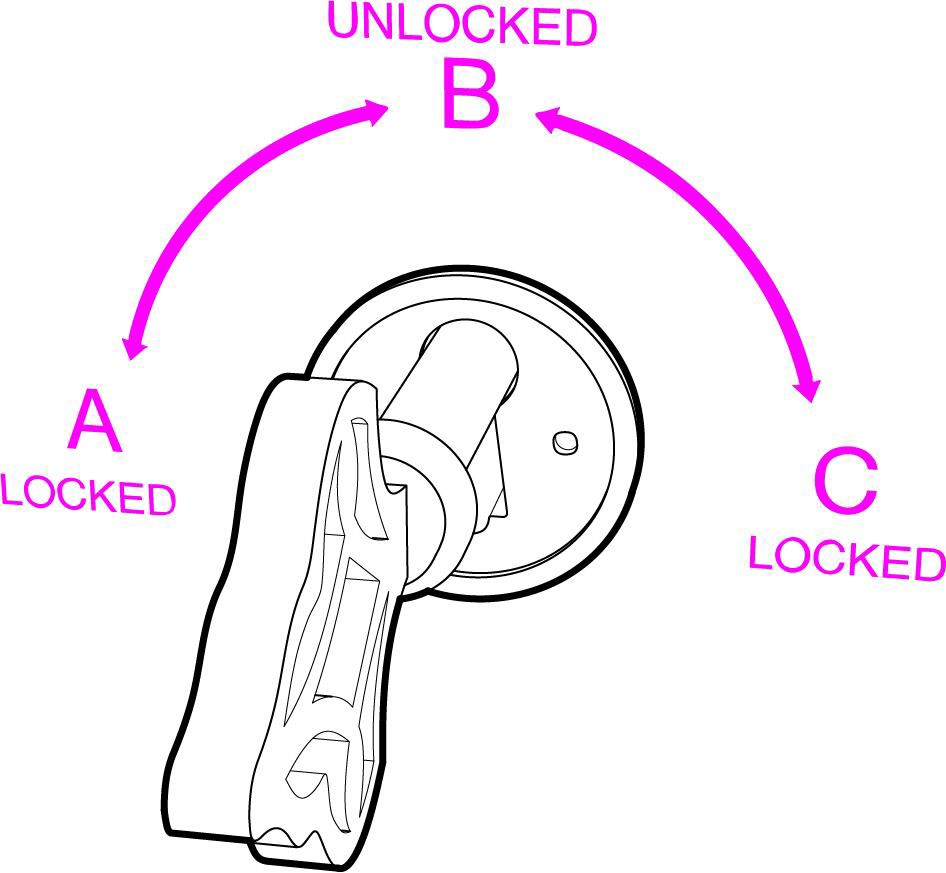
\includegraphics[scale=0.1]{lockUnlock.jpg}
        \caption{Ilustración de criptografía asimétrica\footnotemark{}}
    \end{figure}
    \footnotetext{\bibentry{lockU}}
\end{frame}
